\chapter{Programes per a la calculadora \textsf{HP Prime}}\label{sec:progs-HP}
\index{HP Prime@\textsf{HP Prime}}\index{HP Prime@\textsf{HP Prime}!funcions}

\lstset{
	language=HPPRIME,
	numbers=left,
	frame=lines
}

Es donen en aquest apèndix una sèrie de programes per a la calculadora \textsf{HP Prime} de Hewlett-Packard, els quals són d'interès per resoldre problemes tractats en aquest llibre.

\begin{center}
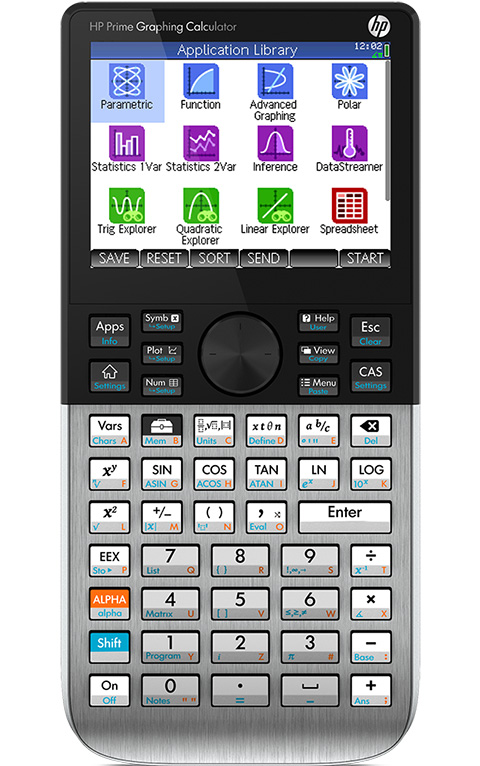
\includegraphics[scale=0.45]{Ape-HP-Prime.jpg}
\end{center}

Aquesta calculadora disposa d'un emulador per a PC que pot descarregar-se de la pàgina de Hewlett-Packard: \href{http://www.hp-prime.de/en/category/6-downloads}{www.hp-prime.de/en/category/6-downloads}.


\section{Electrotècnia}\label{sec:HP_ELC}

La funció \texttt{Z\_Series} utilitza l'equació \eqref{eq:z_serie} per obtenir la impedància sèrie d'una llista d'impedàncies $\cmplx{Z}_1, \cmplx{Z}_2, ...$; les impedàncies poden ser indistintament reals o complexes.

\index{HP Prime@\textsf{HP Prime}!funcions!ZSeries@\texttt{Z\_Series}}
\lstinputlisting[caption={HP Prime --- Funció Z\_Series},linerange={3-7}]{HPPrime/EE_QED.hpprgm}


La funció \texttt{Z\_Parallel} obté la impedància paraŀlel  d'una llista d'impedàncies $\cmplx{Z}_1, \cmplx{Z}_2, ...$; les impedàncies poden ser indistintament reals o complexes. S'utilitza una variant de l'equació \eqref{eq:z_parallel}, la qual dona una millor precisió numèrica.

\index{HP Prime@\textsf{HP Prime}!funcions!ZParallel@\texttt{Z\_Parallel}}
\lstinputlisting[caption={HP Prime --- Funció Z\_Parallel},linerange={9-13}]{HPPrime/EE_QED.hpprgm}


La funció \texttt{Millman} utilitza l'equació \eqref{eq:millman} per obtenir la tensió $\cmplx{U}\ped{NX}$ del punt neutre N d'una llista d'impedàncies connectades en estrella $\cmplx{Z}\ped{AN}, \cmplx{Z}\ped{BN}, \cmplx{Z}\ped{CN}, ...$, respecte d'un punt qualsevol X, a partir de la llista de tensions $\cmplx{U}\ped{AX}, \cmplx{U}\ped{BX}, \cmplx{U}\ped{CX}, ...$ dels extrems d'aquestes impedàncies respecte del mateix punt X; les impedàncies i les tensions poden ser indistintament reals o complexes. És necessària la funció \texttt{Z\_Parallel}, definida anteriorment.

\index{HP Prime@\textsf{HP Prime}!funcions!Millman@\texttt{Millman}}
\lstinputlisting[caption={HP Prime --- Funció Millman},linerange={15-20}]{HPPrime/EE_QED.hpprgm}


La funció \texttt{D\_to\_Y} utilitza l'equació \eqref{eq:Y_D} per transformar una llista de tres impedàncies connectades en triangle $\cmplx{Z}\ped{AB}$, $\cmplx{Z}\ped{BC}$ i  $\cmplx{Z}\ped{CA}$, en una llista de tres impedàncies equivalents connectades en estrella $\cmplx{Z}\ped{AN}$, $\cmplx{Z}\ped{BN}$ i $\cmplx{Z}\ped{CN}$; les impedàncies poden ser indistintament reals o complexes.

\index{HP Prime@\textsf{HP Prime}!funcions!DtoY@\texttt{D\_to\_Y}}
\lstinputlisting[caption={HP Prime --- Funció D\_to\_Y},linerange={22-27}]{HPPrime/EE_QED.hpprgm}


La funció \texttt{Y\_to\_D} utilitza l'equació \eqref{eq:Y_D} per transformar una llista de tres impedàncies connectades en estrella $\cmplx{Z}\ped{AN}$, $\cmplx{Z}\ped{BN}$ i $\cmplx{Z}\ped{CN}$, en una llista de tres impedàncies equivalents connectades en triangle $\cmplx{Z}\ped{AB}$, $\cmplx{Z}\ped{BC}$ i  $\cmplx{Z}\ped{CA}$; les impedàncies poden ser indistintament reals o complexes.

\index{HP Prime@\textsf{HP Prime}!funcions!YtoD@\texttt{Y\_to\_D}}
\lstinputlisting[caption={HP Prime --- Funció Y\_to\_D},linerange={29-34}]{HPPrime/EE_QED.hpprgm}


La funció \texttt{EZS\_U} utilitza les equacions de la secció \vref{sec:EZS} per obtenir la tensió $\cmplx{U}$ d'una càrrega que absorbeix una potència $\cmplx{S}$, quan està connectada a una font de tensió $\cmplx{E}$ a través d'una impedància $\cmplx{Z}$; cadascun d'aquests valors pot ser indistintament real o complex.

\index{HP Prime@\textsf{HP Prime}!funcions!EZSU@\texttt{EZS\_U}}
\lstinputlisting[caption={HP Prime --- Funció EZS\_U},linerange={36-47},label=lst:EZSU]{HPPrime/EE_QED.hpprgm}


La funció \texttt{kcmil\_to\_mm2} utilitza l'equació \eqref{eq:kcmil_mm2} per convertir la secció d'un conductor expressada en \unit{kcmil}, en la seva secció equivalent expressada en \unit{mm^2}.

\index{HP Prime@\textsf{HP Prime}!funcions!kcmiltomm@\texttt{kcmil\_to\_mm2}}
\lstinputlisting[caption={HP Prime --- Funció kcmil\_to\_mm2},linerange={49-53}]{HPPrime/EE_QED.hpprgm}


La funció \texttt{mm2\_to\_kcmil} utilitza l'equació \eqref{eq:kcmil_mm2} per convertir la secció d'un conductor expressada en \unit{mm^2}, en la seva secció equivalent expressada en \unit{kcmil}.

\index{HP Prime@\textsf{HP Prime}!funcions!mmtokcmil@\texttt{mm2\_to\_kcmil}}
\lstinputlisting[caption={HP Prime --- Funció mm2\_to\_kcmil},linerange={55-59}]{HPPrime/EE_QED.hpprgm}


La funció \texttt{AWG\_to\_mm2} utilitza l'equació \eqref{eq:awg_mm2} per convertir la secció d'un conductor expressada segons el seu número AWG, en la seva secció equivalent expressada en \unit{mm^2}.

\index{HP Prime@\textsf{HP Prime}!funcions!awgtomm@\texttt{AWG\_to\_mm2}}
\lstinputlisting[caption={HP Prime --- Funció AWG\_to\_mm2},linerange={61-66}]{HPPrime/EE_QED.hpprgm}


La funció \texttt{mm2\_to\_AWG} utilitza l'equació \eqref{eq:mm2_awg} per convertir la secció d'un conductor expressada en \unit{mm^2}, en la seva secció equivalent expressada segons el seu número AWG; la conversió és aproximada, ja que els números AWG prenen valors discrets.

\index{HP Prime@\textsf{HP Prime}!funcions!mmtoawg@\texttt{mm2\_to\_AWG}}
\lstinputlisting[caption={HP Prime --- Funció mm2\_to\_AWG},linerange={68-73}]{HPPrime/EE_QED.hpprgm}


La funció \texttt{Triangle\_to\_Phasors} obté els tres fasors $\cmplx{U}\ped{AB}$, $\cmplx{U}\ped{BC}$ i $\cmplx{U}\ped{CA}$ que formen un triangle de tensions fase-fase, a partir de les longituds dels tres costats d'aquest triangle $|\cmplx{U}\ped{AB}|$, $|\cmplx{U}\ped{BC}|$ i $|\cmplx{U}\ped{CA}|$. Es pren $\cmplx{U}\ped{AB}$ com a fasor de referència.

\index{HP Prime@\textsf{HP Prime}!funcions!TriangletoPhasors@\texttt{Triangle\_to\_Phasors}}
\lstinputlisting[caption={HP Prime --- Funció Triangle\_to\_Phasors},linerange={75-81},label=lst:TriFas]{HPPrime/EE_QED.hpprgm}


La funció \texttt{LN\_to\_LL} obté els fasors de les tres tensions fase-fase $\cmplx{U}\ped{AB}$, $\cmplx{U}\ped{BC}$ i $\cmplx{U}\ped{CA}$, corresponents als fasors de les tres tensions fase-neutre
$\cmplx{U}\ped{AN}$, $\cmplx{U}\ped{BN}$ i $\cmplx{U}\ped{CN}$.

\index{HP Prime@\textsf{HP Prime}!funcions!LNtoLL@\texttt{LN\_to\_LL}}
\lstinputlisting[caption={HP Prime --- Funció LN\_to\_LL},linerange={83-87},label=lst:FNaFF]{HPPrime/EE_QED.hpprgm}


La funció \texttt{LL\_to\_LN} obté els fasors de les tres tensions fase-neutre $\cmplx{U}\ped{AN}$, $\cmplx{U}\ped{BN}$ i $\cmplx{U}\ped{CN}$, corresponents a tres impedàncies $\cmplx{Z}\ped{AN}$, $\cmplx{Z}\ped{BN}$ i $\cmplx{Z}\ped{CN}$ connectades en estrella a  les tres tensions fase-fase
$\cmplx{U}\ped{AB}$, $\cmplx{U}\ped{BC}$ i $\cmplx{U}\ped{CA}$. És necessària la funció \texttt{Z\_Parallel}, definida anteriorment.

\index{HP Prime@\textsf{HP Prime}!funcions!LLtoLN@\texttt{LL\_to\_LN}}
\lstinputlisting[caption={HP Prime --- Funció LL\_to\_LN},linerange={89-93},label=lst:FFaFN]{HPPrime/EE_QED.hpprgm}


La funció \texttt{LL\_to\_LG} obté els fasors de les tres tensions fase-neutre $\cmplx{U}\ped{AG}$, $\cmplx{U}\ped{BG}$ i $\cmplx{U}\ped{CG}$ que tenen el punt neutre G en el baricentre del triangle format pels fasors de  les tres tensions fase-fase
$\cmplx{U}\ped{AB}$, $\cmplx{U}\ped{BC}$ i $\cmplx{U}\ped{CA}$. És un cas particular de la funció anterior, quan les tres impedàncies són idèntiques.

\index{HP Prime@\textsf{HP Prime}!funcions!LLtoLG@\texttt{LL\_to\_LG}}
\lstinputlisting[caption={HP Prime --- Funció LL\_to\_LG},linerange={95-100},label=lst:FFaFG]{HPPrime/EE_QED.hpprgm}


La funció \texttt{ABC\_to\_A012} utilitza l'equació \eqref{eq:c_sim_mat1} per obtenir els tres fasors de seqüència
$\cmplx{A}_0$, $\cmplx{A}_1$ i  $\cmplx{A}_2$ corresponents als tres fasors $\cmplx{A}$, $\cmplx{B}$ i $\cmplx{C}$.

\index{HP Prime@\textsf{HP Prime}!funcions!ABCtoA012@\texttt{ABC\_to\_A012}}
\lstinputlisting[caption={HP Prime --- Funció ABC\_to\_A012},linerange={102-107},label=lst:ABCaA012]{HPPrime/EE_QED.hpprgm}


La funció \texttt{A012\_to\_ABC} fa el càlcul  invers de la funció anterior, i utilitza l'equació \eqref{eq:c_sim_mat} per obtenir els tres fasors
$\cmplx{A}$, $\cmplx{B}$ i $\cmplx{C}$  corresponents als tres fasors de seqüència
$\cmplx{A}_0$, $\cmplx{A}_1$ i  $\cmplx{A}_2$.

\index{HP Prime@\textsf{HP Prime}!funcions!A012toABC@\texttt{A012\_to\_ABC}}
\lstinputlisting[caption={HP Prime --- Funció A012\_to\_ABC},linerange={109-114},label=lst:A012aABC]{HPPrime/EE_QED.hpprgm}


La funció \texttt{AN12\_to\_AB12} utilitza les equacions  \eqref{eq:c_sim_a3} i \eqref{eq:c_sim_b3} per obtenir els dos fasors de tensions de seqüència fase-fase $\cmplx{U}\ped{AB,1}$ i  $\cmplx{U}\ped{AB,2}$ a partir dels dos fasors de tensions de seqüència fase-neutre $\cmplx{U}\ped{AN,1}$ i $\cmplx{U}\ped{AN,2}$.

\index{HP Prime@\textsf{HP Prime}!funcions!AN12toAB12@\texttt{AN12\_to\_AB12}}
\lstinputlisting[caption={HP Prime --- Funció AN12\_to\_AB1},linerange={116-120},label=lst:AN12aAB12]{HPPrime/EE_QED.hpprgm}


La funció \texttt{AB12\_to\_AN12} fa el càlcul invers de la funció anterior, i utilitza les mateixes equacions  \eqref{eq:c_sim_a3} i \eqref{eq:c_sim_b3} per obtenir els dos fasors de tensions de seqüència fase-neutre $\cmplx{U}\ped{AN,1}$ i $\cmplx{U}\ped{AN,2}$ a partir dels dos fasors de tensions de seqüència fase-fase $\cmplx{U}\ped{AB,1}$ i  $\cmplx{U}\ped{AB,2}$:

\index{HP Prime@\textsf{HP Prime}!funcions!AB12toAN12@\texttt{AB12\_to\_AN12}}
\lstinputlisting[caption={HP Prime --- Funció AB12\_to\_AN12},linerange={122-126},label=lst:AB12aAN12]{HPPrime/EE_QED.hpprgm}


\section{Matemàtiques}

La funció \texttt{Polynomial\_Interpolation} obté l'ordenada interpolada $y$ corresponent a una abscissa $x$, a partir d'un conjunt  de punts $(x_1,y_1)$, $(x_2,y_2)$, ..., $(x\ped{n},y\ped{n})$. S'utilitza una interpolació polinòmica, obtenint els mateixos resultats que amb el mètode descrit en la secció \vref{sec:poli_lagr}; el grau del polinomi és igual a $n-1$.

\index{HP Prime@\textsf{HP Prime}!funcions!PolynomialInterpolation@\texttt{Polynomial\_Interpolation}}
\lstinputlisting[caption={HP Prime --- Funció Polynomial\_Interpolation},linerange={3-10}]{HPPrime/Math_QED.hpprgm}


La funció \texttt{Polynomial\_Interpolation\_2D} obté el valor interpolat $z$ corresponent a un punt $(x, y)$, a partir d'un conjunt de punts $(x\ped{1}, x\ped{2}, ... x\ped{n})$, d'un conjunt de punts $(y\ped{1}, y\ped{2}, ... y\ped{m})$, i d'una matriu de valors $(z\ped{11}, z\ped{12}, ..., z\ped{1n})$,
$(z\ped{21}, z\ped{22}, ..., z\ped{2n})$, ..., $(z\ped{m1}, z\ped{m2}, ..., z\ped{mn})$. S'utilitzen  interpolacions polinòmiques, aconseguint els mateixos resultats que amb el mètode descrit en la secció \vref{sec:poli_lagr}; el grau dels polinomis és igual a $n-1$ i $m-1$.
És necessària la funció \texttt{Polynomial\_Interpolation}, definida anteriorment.

\index{HP Prime@\textsf{HP Prime}!funcions!PolynomialInterpolation2D@\texttt{Polynomial\_Interpolation\_2D}}
\lstinputlisting[caption={HP Prime --- Funció Polynomial\_Interpolation\_2D},linerange={12-31}]{HPPrime/Math_QED.hpprgm}


La funció \texttt{Trapezoidal\_Rule} utilitza l'equació  \eqref{eq:trap-uneven} per obtenir la integral entre $x_1$ i $x_n$ d'un conjunt  de punts $(x_1,y_1)$, $(x_2,y_2)$, ..., $(x\ped{n},y\ped{n})$, utilitzant la regla dels trapezis.

\index{HP Prime@\textsf{HP Prime}!funcions!TrapezoidalRule@\texttt{Trapezoidal\_Rule}}
\lstinputlisting[caption={HP Prime --- Funció Trapezoidal\_Rule},linerange={33-45}]{HPPrime/Math_QED.hpprgm}
